
\subsection{Motorik der Kopfmuskulatur} \index{Motorik! Kopf}
Neben der Muskulatur der Augen lassen sich die restliche Muskeln des Kopfes, sowie seine Innervation grob in vier Gruppen einteilen: Die Gesichtsmuskulatur, die Kaumuskulatur, die Zungenmuskulatur und die Pharynx- und Kehlkopfmuskulatur. Jeder dieser Muskeleinheiten wird durch ein bestimmtes Kerngebiet über die Hirnnerven kontrolliert. Alle Kerngebiete, die an der Kontrolle der Kopfmuskulatur beteiligt, sind erhalten Afferenzen aus dem Motorkortex der Großhirnrinde. Im Folgenden werden die einzelnen Gruppen getrennt beschrieben.

\subsubsection*{Gesichtsmuskulatur}
Die Muskulatur der Gesichtes wird über den VII. Hirnnerv \textbf{Nervus facialis} \index{Hirnnerven! 07. N. facilis} gesteuert. Dieser Nerv besteht allerdings nicht nur aus motorischen Fasern, sondern auch aus sensorischen und parasympathischen Komponenten. Den Hirnstamm verlässt er auf der ventrolateralen Seite des caudalen Pons. Dieser Bereich wird auch Kleinhirnbrückenwinkel genannt. Die sensorischen und parasympathischen Fasern können von den motorischen Fasern als eigener Nervenstrang abgegrenzt werden. Er liegt mehr lateral und wird auch oftmals als Nervus intermedius bezeichnet. Der medial verlaufende Fazialisnerv besteht nur aus motorischen Axonen, die ihren Ursprung im \textit{Nucleus nervi facialis} \index{Nucleus! nervi facialis} des Pons nehmen (Abb. \ref{fig:kerne_kopfmotorik}~C). Von dort ziehen die Fasern typischerweise dorsokranial um den Nucleus abducens, unterhalb des vierten Ventrikels, herum. Dabei bilden sie die spezifische Struktur des Colliculus facialis (inneres Fazialisknie) am Boden der Rautengrube (Abb.~\ref{fig:nervus-facialis}). Über diesen motorischen Strang wird vor allem die mimische Gesichtsmuskulatur innerviert. Zusätzlich wird auch der Musculus stapedius des Mittelohrs über den Fazialisnerv aktiviert \textsuperscript{\cite[Kap.~10][5]{crossman2014neuroanatomy, trepel2011neuroanatomie}}. \\
Der Ncl. n. facialis erhält den Großteil seiner Afferenzen aus der Großhirnrinde. Dabei ist zu beachten, dass diese Fasern nicht ausschließlich vom Motorcortex stammen. Es sind vier weitere Bereiche des Cortex mit unterschiedlichen Funktionen bekannt. Der Motorkortex steuert zusammen mit einem Gebiet im lateroventralen präfrontalen Cortex willkürlich die mimische Muskulatur der unteren Gesichtshälfte. Für die willkürliche Kontrolle der oberen Gesichtshälfte ist ein Bereich im supplementärmotorischen Cortex zuständig. Innerhalb des Gyrus cinguli existieren zwei Zonen, die jeweils die emotional ausgelöste Bewegung der oberen oder unteren Gesichtshälfte initiieren. Die untere Gesichtshälfte wird dabei immer von der contralateralen Seite der Großhirnrinde gesteuert, wohingegen die obere unter bilateraler Kontrolle steht \textsuperscript{\cite[Kap.~9]{trepel2011neuroanatomie}}. \\
Ein kleiner Teil der Afferenzen des Ncl. n. facialis stammt auch aus Bereichen des Hirnstammes um Reflexreaktionen zu vermitteln. Dazu zählt zum einen der Lidschlussreflex, als Antwort auf visuelle und taktile Stimuli, der von den Colliculi superiores und dem sensorischen Kern des Trigeminusnerves gleichermaßen vermittelt wird. Zum anderen wird der Mittelohrreflex als Reaktion auf laute Geräusche ausgehend vom Nucleus olivaris superior über den Facialiskern induziert \textsuperscript{\cite[Kap.~10]{crossman2014neuroanatomy}}. \\
Innerhalb des Ncl. n. facialis der Ratte lassen sich vier Kerngebiete - \textbf{lateraler}, \textbf{dorsolateraler}, \textbf{intermediärer} und \textbf{medialer Subnucleus} - durch eine Schicht weißer Substanz voneinander abgrenzen. Diese Unterteilung erstreckt sich über die rostro-caudale Ausbreitung des Kerns. Die Motorneurone der Ohren und der Halsmusklulatur entstammen dem medialen Gebiet. Aus der intermediären Region entspringt die periorale Kontrolle. Die Mundregion wird über den dorsolateralen Subnucleus gesteuert. Die Motorneurone, die das Vibrissenfeld innervieren, stammen aus dem lateralen Bereich. Der Großteil dieser Fasern ist für die Kontrolle der inneren Vibrissenmuskulatur, die jeden Vibrissenfollikel umgibt, zuständig. Es wird angenommen, dass eine Vibrisse von ungefähr 25 Motorneuronen innerviert wird. Die Fasern der dorsal gelegenen Vibrissen liegen lateraler als die Fasern der ventralen Vibrissen. Motorneurone, die für die Steuerung der äußeren Vibrissenmuskulatur inklusive des Musculus levator nasolabialis	zuständig sind, entspringen dem dorsolateralen Kerngebiet \textsuperscript{\cite[Kap.~11]{paxinos2014rat}}.   


\begin{figure}[H]
    \centering
    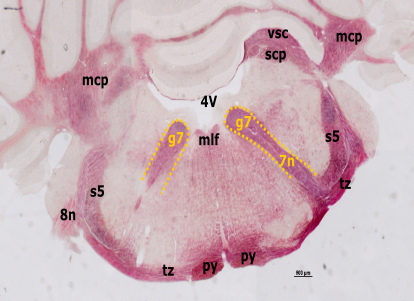
\includegraphics[width=0.8\textwidth]{pictures/Bilder_Laura/facialis_Nerv_F09_1png.png}
    \caption[Verlauf des Nervus facialis]{\textbf{Verlauf des Nervus facialis.} Zu erkennen ist der charakteristische Verlauf des Nervus facialis (7n). Seine Fasern ziehen dorsokranial unterhalb des vierten Ventrikels (4V) um den Nucleus abducens und bilden dabei das Knie des Facialisnervs (g7). Außerdem in der Abbildung zu erkennende Fasertrakte: Pryramidentrakt (py), Trapezkörper (tz), sensorische Wurzel des Trigeminusnervs (s5), Fasciculus longitudinalis medialis (mlf), mittlerer Kleinhirnstiel (mcp), superiorer Kleinhirnstiel (scp) und ventraler Spinocerebellarer Trakt (vsc). Faser-Färbung (F09-1).}
    \label{fig:nervus-facialis}
\end{figure}

\subsubsection*{Kaumuskulatur} 
Die motorischen Fasern zur Innervation der Kaumuskulatur gehen aus dem \textit{Nucleus motorius nervi trigemini} \index{Nucleus! motorius nervi trigemini} hervor. Dieses Kerngebiet liegt im Tegmentum pontis medial des Nucleus principalis nervi trigemini (Abb.~\ref{fig:kerne_kopfmotorik}~D). Die Fasern, die aus diesem Bereich hervorgehen, gehören zu dem V. Hirnnerv (\textbf{Nervus trigeminus})\index{Hirnnerven! 05. N. trigeminus}. Dieser Nerv setzt sich hauptsächlich aus sensorischen Fasern zusammen, da er der wichtigste sensorische Nervs des Kopfes ist. Die motorischen Fasern machen nur einen geringen Anteil aus. Sie verlassen den Hirnstamm zusammen in der Mitte des Pons als dickster Hirnstammnerv und laufen von dort ventrolateral am Pons entlang. Der motorische Anteil ist für die Innervation einiger Muskeln zuständig. Die wichtigste ist die Kaumuskulatur. Dazu zählen der Musculus masseter und der Musculus temporalis, die für das Schließen des Kiefers zuständig sind, sowie der Musculus pterygoideus medialis und Musculus pterygoideus lateralis, welche den Kiefer wieder öffnen \textsuperscript{\cite[Kap.~10]{crossman2014neuroanatomy}}.

\subsubsection*{Zungenmuskulatur}
Die Muskulatur der Zunge wird durch den XII. Hirnnerv \textbf{Nervus hypoglossus} \index{Hirnnerven! 12. N. hypoglossus} innerviert. Er besteht nur aus motorischen Fasern, die alle dem \textit{Nucleus nervi hypoglossi} \index{Nucleus! nervi hypoglossi} entstammen. Dieses Kerngebiet ist in der Medulla oblongata paramedian unterhalb des vierten Ventrikels als langgestreckte Zellsäule zu finden (Abb.~\ref{fig:kerne_kopfmotorik}~A,B). Von dort verlaufen die Fasern ventral entlang der Medulla, bis sie ventrolateral zwischen der Pyramide und der Olive den Hirnstamm verlassen. Der N. hypoglossus ist für die Innervation der äußeren und inneren Zungenmuskulatur zuständig. Mit dieser Muskulatur lässt sich sowohl die Zunge bewegen, als auch ihre Form verändern \textsuperscript{\cite[Kap.~10]{crossman2014neuroanatomy}}.

\subsubsection*{Pharynx- und Kehlkopfmuskulatur}
Die Muskulatur des Pharynx und des Kehlkopfes wird über wird über das Kerngebiet des \textit{Nucleus ambiguus} \index{Nucleus! ambiguus} innerhalb der Medulla oblongata kontrolliert. Dieser speziell-viszeromotorische Kern sendet Fasern über zwei Hirnnerven, den \textbf{Nervus glossopharyngeus} (IX.) \index{Hirnnerven! 09. N. glossopharyngeus} und den \textbf{Nervus vagus} (X.)\index{Hirnnerven! 10. N. vagus}, zur Muskulatur um sie zu innervieren. Der N. glossopharyngeus besteht zum Großteil aus sensorischen und parasympathischen Fasern. Der motorische Anteil ist sehr gering. Insgesamt entspringen diese Fasern aus vier unterschiedlichen Kerngebieten. Der Ncl. abmiguus ist einer davon. Aus dem rostralen Bereich des Ncl. ambiguus stammen die Axone, welche als motorischer Anteil innerhalb des N. glossopharyngeus zur Schlund- und Gaumensegelmuskulatur ziehen. Diese Fasern sind für die Innervation eines Muskels, des Musculus stylopharyngeus, zuständig, welcher für das Schlucken benötigt wird. \\
Auch der N. vagus ist ein gemischter Nerv, der sich aus sensorischen, parasympathischen und motorischen Fasern zusammensetzt, die aus vier unterschiedlichen Kernen stammen. Die motorischen Fasern stammen aus dem Ncl. ambiguus der Medulla. Sie innervieren Muskulatur der Gaumensegel, des Pharynx, des Larynx und auch des oberen Ösophagus. Damit nimmt der Ncl. ambiguus und der N. vagus eine wichtige Funktion in der Kontrolle des Sprechens und Schluckens ein \textsuperscript{\cite[Kap.~10]{crossman2014neuroanatomy}, \cite[5]{trepel2011neuroanatomie}}.       

\begin{figure}[H]
    \centering
    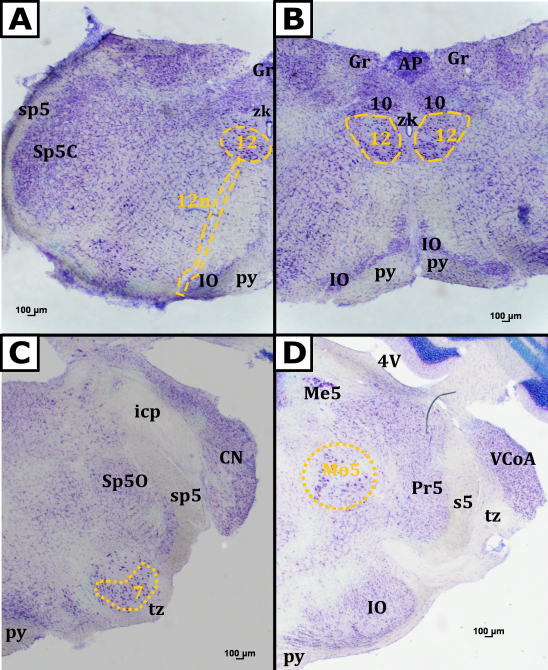
\includegraphics[width=0.8\textwidth]{pictures/Bilder_Laura/Kerne_motorik_kopf_N01_3_N01_4_N06_4_N09_3.png}
    \caption[Motorische Kerne des Kopfes]{\textbf{Motorische Kerne des Kopfes.} Die Schnitte sind von caudal nach rostral angeordnet. Die Schnitte A und~B zeigen den Verlauf des Nucleus nervi hypoglossi im Abstand von 150~$\upmu$m. \textbf{A:} Der Nucleus nervi hypoglossi (12) ist in der Medulla oblongata medial unterhalb des Zentralkanals (zk) lokalisiert. Von ihm zieht die Wurzel des Nervus hypoglossus (12n) nach ventral, wo sie dann zwischen der Pyramide (py) und der unteren Olive (IO) den Hirnstamm verlassen. Lateral zu erkennen ist der caudale Nucleus spinalis nervi trigemini (Sp5c) und der dazugehörige Trakt des spinalen Trigeminusnerves (sp5). Dorsal ist der Nucleus gracilis (Gr) zu sehen. Nissl-Färbung (N01-3). \textbf{B:} Oberhalb des Ncl. n. hypoglossi (12) ist der dorsale motorische Kern des Vagusnervs (10) zu erkennen. Dorsal ist die Area postrema (AP) zu sehen. Nissl-Färbung (N01-4). \textbf{C:} Der Nucleus facialis (7) liegt ventrolateral innerhalb des Pons. Außerdem lateral zu erkennen: Trapezkörper (tz), oraler Bereich des Nucleus spinalis nervi trigemini (Sp5o), Nucleus cochlearis (CN) und der inferiore Kleinhirnstiel (icp). Nissl-Färbung (N06-4). \textbf{D:} Der Nucleus motorius nervi trigemini (Mo5) liegt medial im Tegmentum pontis unterhalb des vierten Ventrikels (4V) und des Nucleus mesencephali (Me5). Außerdem lateral zu erkennen: Nucleus principalis (Pr5), sensorische Wurzel des Trigeminusnervs (s5) und der anteriore Bereich des ventralen Nucleus cochlearis (VCoA). Nissl-Färbung (N09-3).}
    \label{fig:kerne_kopfmotorik}
\end{figure}